%!TEX root = ../thesis.tex
\chapter{Area covered in the first-order model\label{app:area}}
\label{sec:2dmodel:1starea}
Rather than consider the amount of new area covered, we determine the amount of overlap between the two areas, and subtract this from the sum of the two areas at the end.
\begin{figure}[h!]
	\centering
	\subfloat[{Case 1: Large turning-angle with large $\ell_2$}]{%
		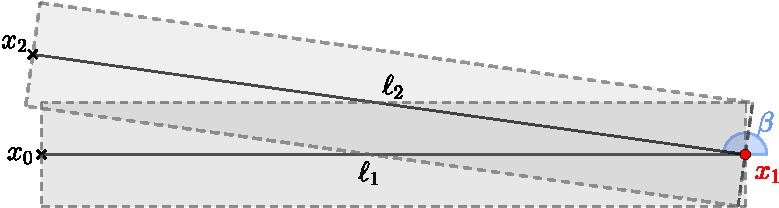
\includegraphics[width=.42\textwidth]{2D-1stOrderApproximation_rectangles_largeTA_largel2_nolabels-crop}}\hfill
	\subfloat[{Case 2: Large turning-angle with small $\ell_2$}]{%
		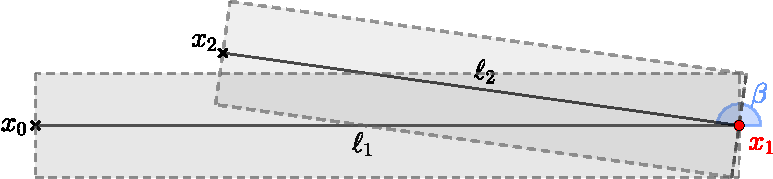
\includegraphics[width=.42\textwidth]{2D-1stOrderApproximation_rectangles_largeTA_smalll2_nolabels-crop}}\\
	\subfloat[Case 3: Medium turning-angle]{%
		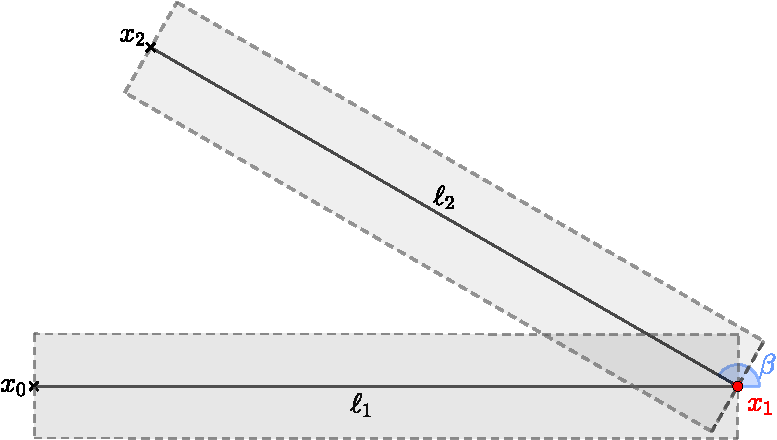
\includegraphics[width=.42\textwidth]{2D-1stOrderApproximation_rectangles_mediumTA_nolabels-crop}}\hfill
	\subfloat[Case 4: Small turning-angle]{%
		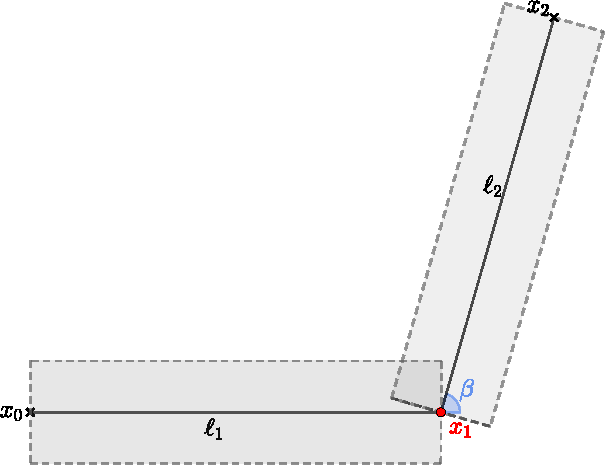
\includegraphics[width=.42\textwidth]{2D-1stOrderApproximation_rectangles_smallTA_nolabels-crop}}
	\caption[The four different cases for the turning-angle that we consider when determining the area of overlap]{The four cases that need to be considered to determine the overlapping area between two steps, with different turning-angles giving rise to different cases. When the turning-angle is large, which of case $1$ or case $2$ arise depends on the relative sizes of $\ell_1$ and $\ell_2$. When $\ell_2$ is sufficiently small, case $3$ becomes case $2$. Four more cases exist for turning-angles greater than $\pi$, although these are mirrors of the four cases above.}\label{fig:2d_model:firstorder:fourcasesappendix}
\end{figure}

\FloatBarrier
\paragraph{Case 1: Large turning-angle, large $\ell_2$}
\FloatBarrier
\begin{figure}[h!]
	\centering
	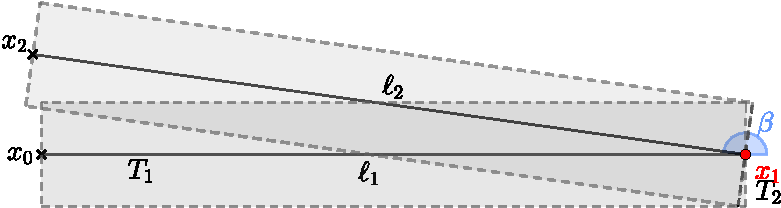
\includegraphics[width=1.0\textwidth]{2D-1stOrderApproximation_rectangles_largeTA_largel2-crop}
	\caption[Case 1: A large turning angle and large step]{Case 1: A large turning-angle and a large $\ell_2$. The bottom left triangle, $T_1$, and the bottom-right triangle, $T_2$, are labelled.}
	\label{fig:2d_model:firstorder:case1}
\end{figure}

For large turning-angles and large $\ell_2$, a large amount of overlap occurs. We consider a turning-angle to be large when the bottom parallel line to $\ell_2$ crosses the top parallel line of $\ell_1$. For this case, we require $\ell_2$ to be large enough relative to $\ell_1$ so that the $\ell_2$ rectangle extends out of the end of the $\ell_1$ rectangle, as it does in \cref{fig:2d_model:firstorder:case1}. The threshold length at which this occurs is when the horizontal component of $\ell_2$ is larger than $\ell_1$, which implies that we require $\ell_1 < -\ell_2 \cos (\beta)$. 

Note that there is not a clear transition between case $1$ and case $2$ at $\ell_1 = -\ell_2 \cos(\beta)$, but rather, there is a separate case entirely, since when $\ell_1$ is slightly smaller than $-\ell_2 \cos(\beta)$, geometry will arise that does not fall into either of the two cases. In this transition, both of the left-most corners will be outside of the $\ell_1$ rectangle while the line between the corners is within the rectangle, meaning a small triangle shaped area will be counted when it shouldn't. This can be seen in \cref{fig:2d_model:firstorder:case1-case2-threshold}. However, since this occurs only in a very specific situation, and the effect is very small, we disregard this and simply assume that case $2$ becomes case $1$ once $\ell_1 < -\ell_2 \cos(\beta)$.

\begin{figure}[h!]
	\centering
	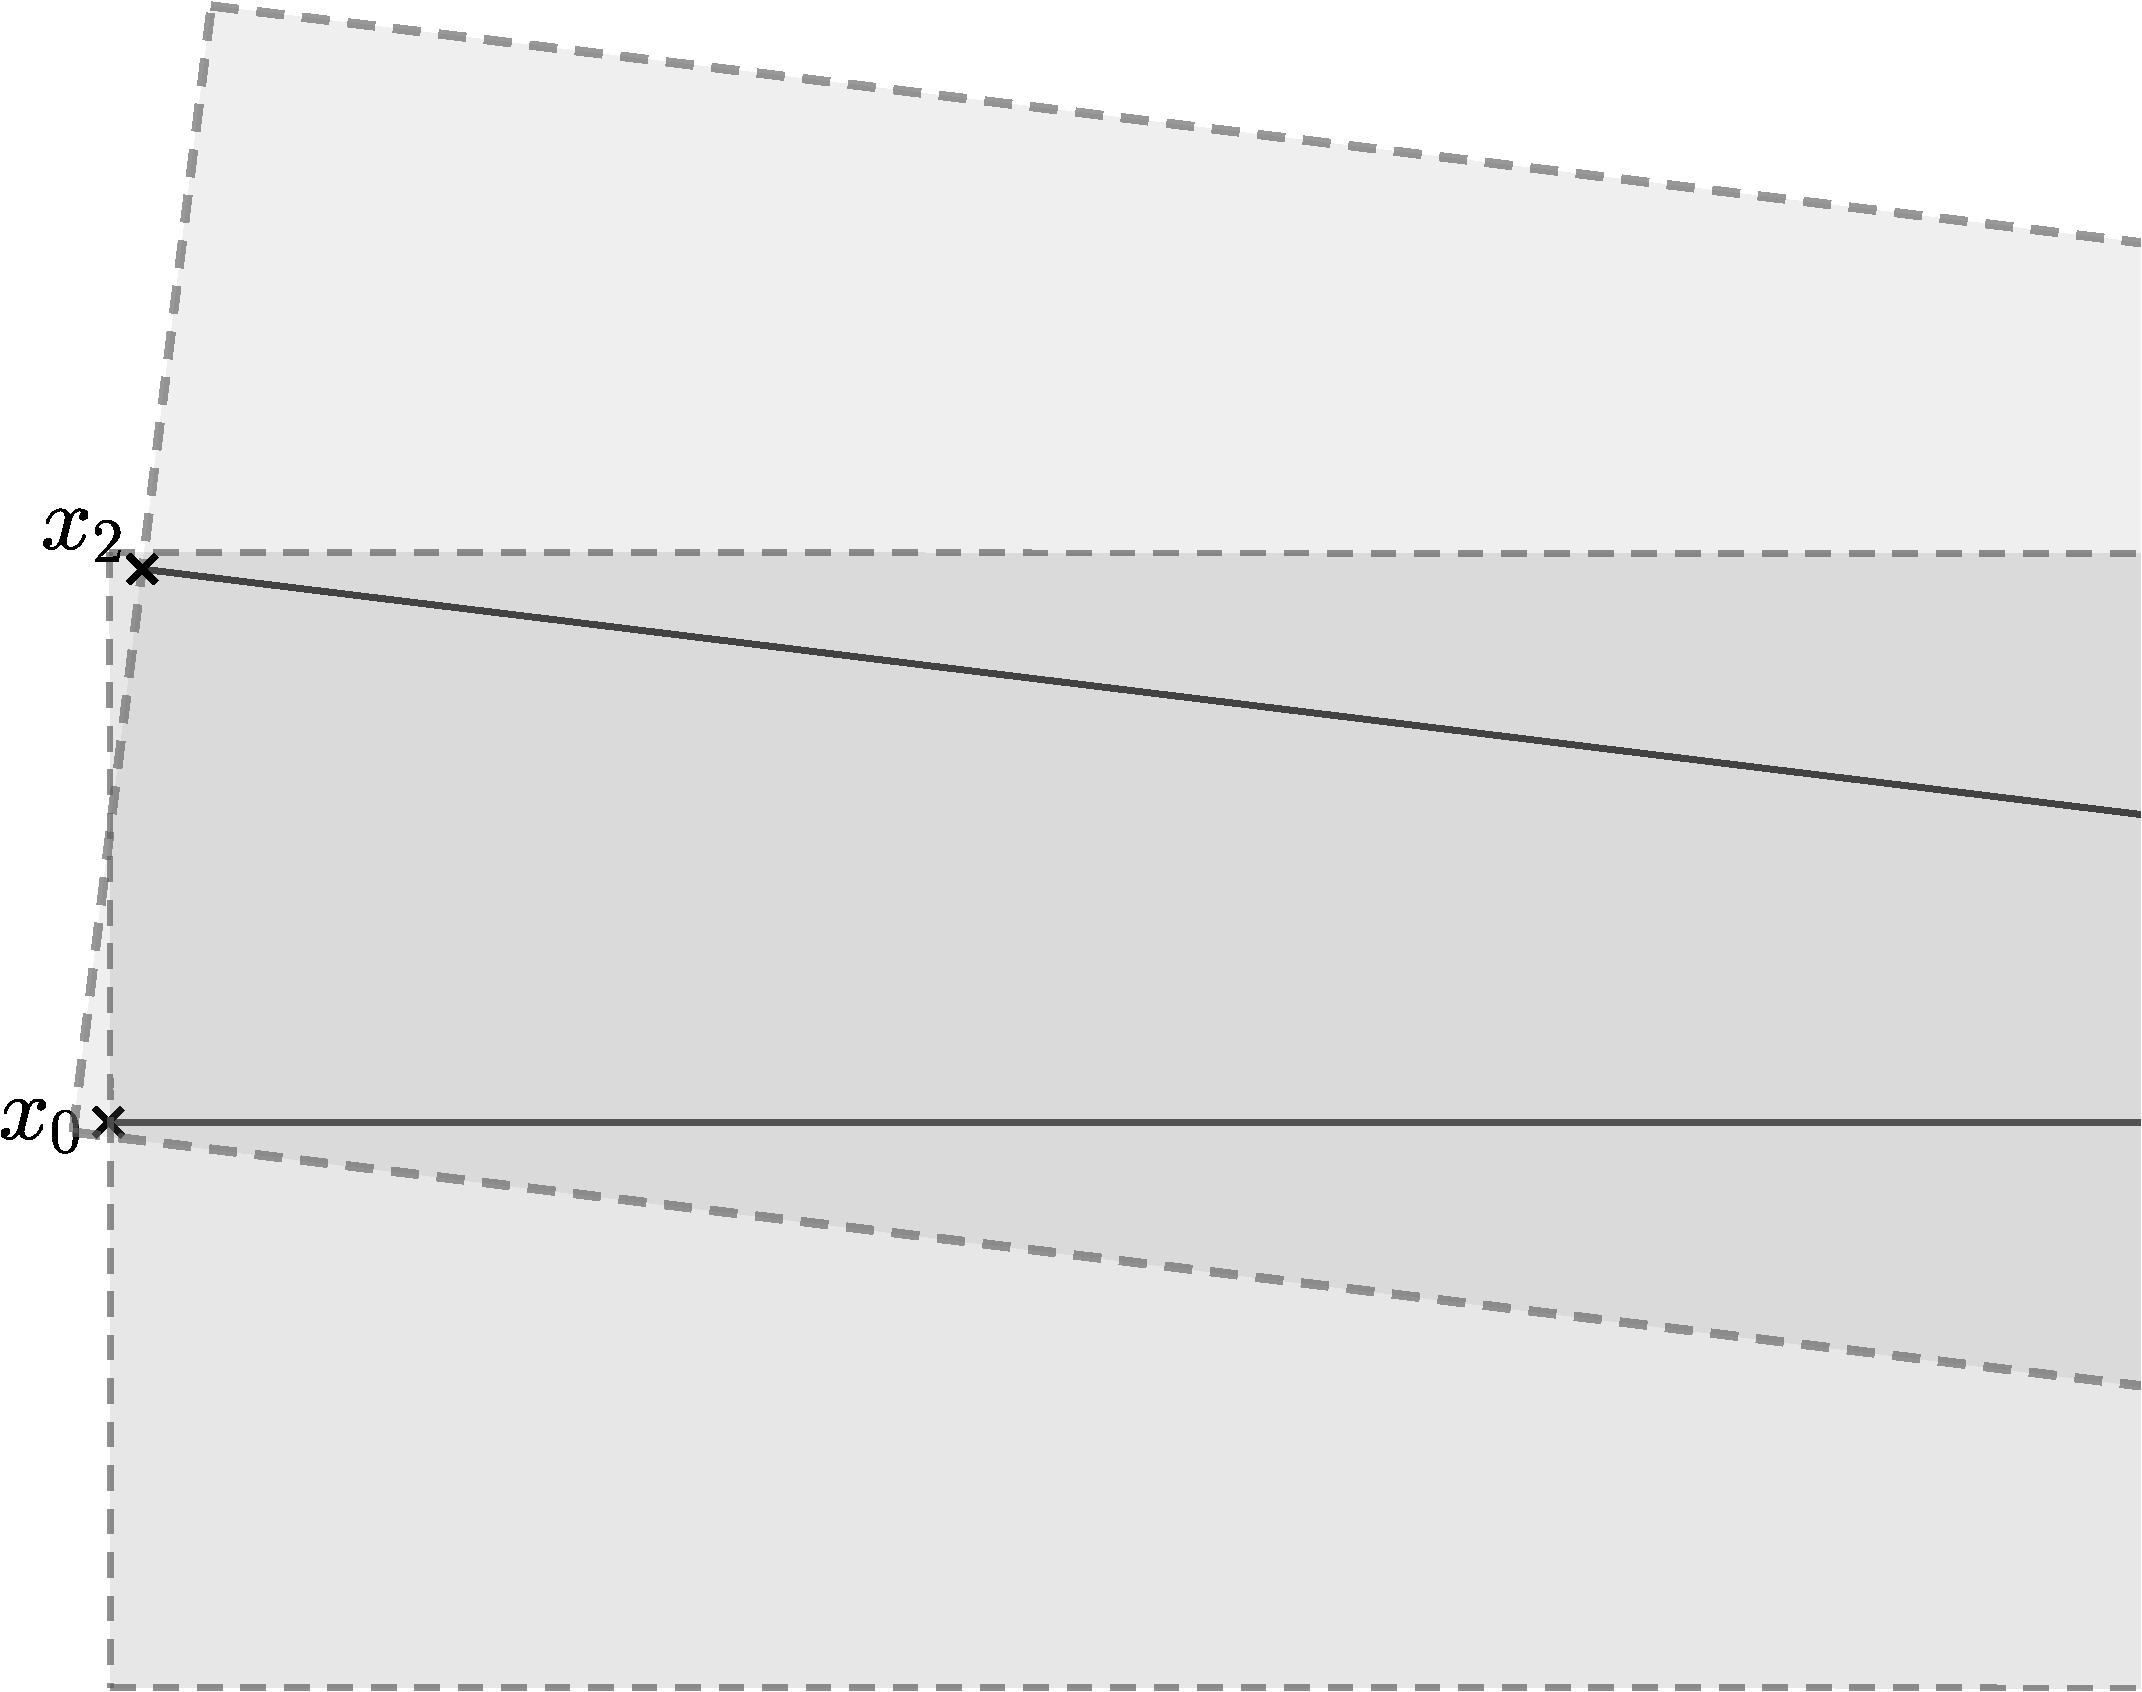
\includegraphics[width=1.0\textwidth]{2D-1stOrderApproximation_rectangles_largeTA_mediuml2-crop}
	\caption[There is no clear threshold between case $1$ and case $2$, although we assume that there is since the introduced error is only small]{There is not a clear threshold between case $1$ and case $2$, as can be seen in the above figure, which does not fall into either case. We assume that there is a clear threshold between the two cases, at the point when the bottom left corner of the $\ell_2$ rectangle exits the $\ell_1$ rectangle. The error caused by doing this will be small since the only difference is the small triangle on the left being counted as overlap when it should not be.}
	\label{fig:2d_model:firstorder:case1-case2-threshold}
\end{figure}

For case $1$, rather than find the area of overlap, it is easier to find the area of the $\ell_1$ rectangle that does not have any overlap.  This is the large right-angled triangle at the bottom, as well as the small right-angled triangle at the bottom right, which we denote $T_1$ and $T_2$ respectively. Note that the non-overlapping area isn't entirely made up of these two triangles since they do not perfectly meet the bottom of the $\ell_1$ rectangle, as seen in \cref{fig:2d_model:firstorder:case1-triangles}, although we assume that they do to avoid extra complications at the cost of a very small amount of accuracy. 

\begin{figure}[h!]
	\centering
	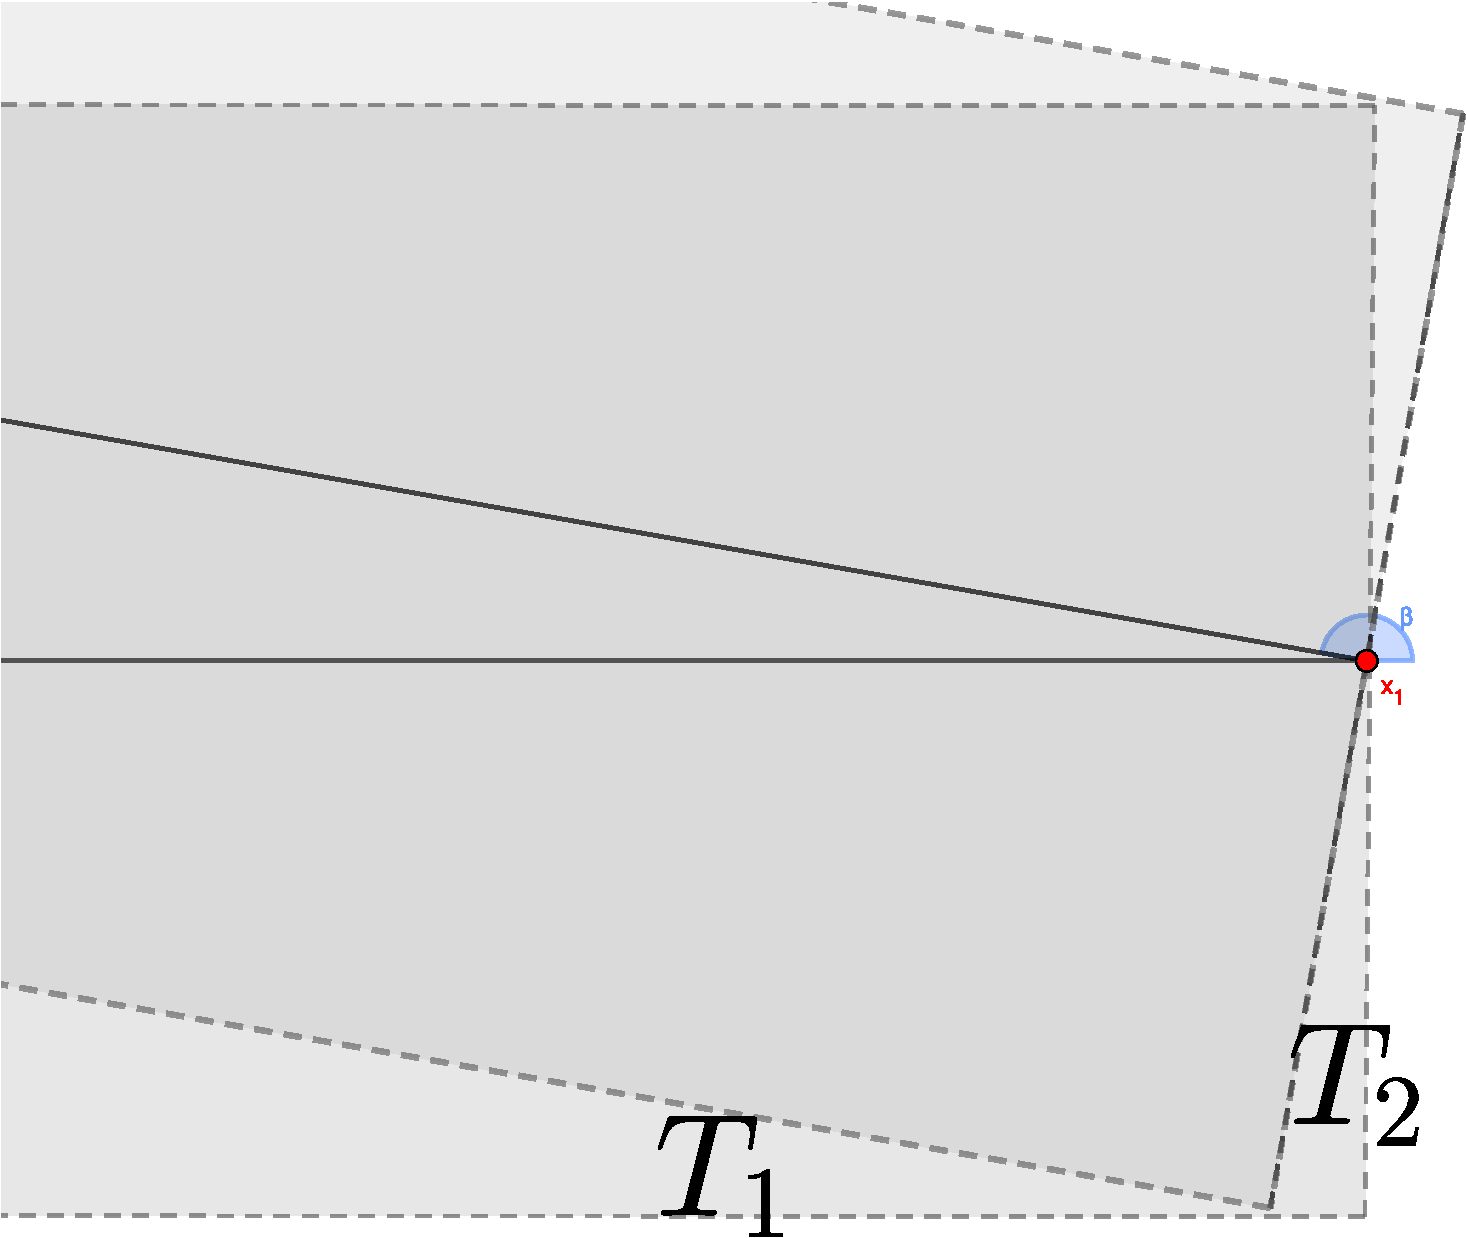
\includegraphics[width=1.0\textwidth]{2D-1stOrderApproximation_rectangles_largeTA_largel2_triangles-crop}
	\caption[A simplification that must be made in order to find the area for case 1]{The total unshaded area is not exactly $T_1 + T_2$, since the triangle $T_1$ does not meet the bottom line. The difference is so small that we assume they do meet, since it simplifies the calculations at the expense of very little error.}
	\label{fig:2d_model:firstorder:case1-triangles}
\end{figure}



The height of the triangle $T_2$ is $r_v$ and the angle at $x$ is $\pi-\beta$, and so the base must be $r_v\tan(\pi-\beta)$. Thus we get
\[A_{T_2} = \frac{-r_v^2}{2} \tan(\beta). \]
The base of triangle $T_1$ has length $\ell_1-r_v\tan(\pi-\beta) = \ell_1+r_v\tan(\beta)$, and the angle at the bottom-right of $T_1$ is $\pi - \beta$. The height of $T_1$ must therefore be
\[\tan(\pi-\beta) = h/(\ell_1+r_v\tan(\beta)) \implies h = -\ell_1 \tan(\beta)-r_v\tan^2(\beta). \]
The area of triangle $T_1$ is
\[A_{T_1} =(\ell_1+r_v\tan(\beta))(-\ell_1 \tan(\beta)-r_v\tan^2(\beta))/2 = \frac{-\left(\ell_1^2 \tan(\beta) + 2r_v\ell_1 \tan^2(\beta)+ r_v^2\tan^3(\beta)\right)}{2}, \]
and so the total area of overlap is
\begin{align*}
A_{\text{overlap}} &= 2 r_v \ell_1 - A_{T_1} - A_{T_2}\\
&=\frac{\ell_1^2 \tan(\beta) + 2r_v \ell_1(2+\tan^2(\beta))  + r_v^2 \tan^3(\beta)}{2}.
\end{align*}

\iffalse
Now, we determine the threshold angle at which the large turning-angle of case $1$ becomes a medium turning-angle of case $3$. We first determine the length along $\ell_2$ at which the line crosses the top edge of the $\ell_1$ rectangle. The top right of the $\ell_1$ rectangle is a right angle triangle with height $r_v$ and bottom right angle $\beta-\pi/2$. The hypotenuse must therefore be of length $r_v/\sin(\beta)$. The distance between the intersection of $\ell_2$ with the top of the $\ell_1$ rectangle, and the point $x_2$ must therefore be $\ell_2-r_v/\sin(\beta)$. We can construct a right angle triangle by drawing a line vertically down from $x_2$, which must have height $\ell_2\sin\beta-r_v$. The bottom left corner of the $\ell_2$ rectangle is a vertical distance of $-r_v\cos\beta$ below $x_2$. Thus, the height of the bottom left corner above $x_1$ is $\ell_2\sin\beta-r_v+r_v\cos\beta$. Then, the threshold angle is when this corner is above $x_1$ by $r_v$, and so we rearrange to get 
\fi

We can also use the height of triangle $T_1$ to determine the threshold angle at which the case of a large turning-angle becomes a medium turning-angle, and vice versa. When the height is greater than the width of the rectangle, $2r_v$, the turning-angle is considered medium. Thus, the threshold angle is
\[-\ell_1 \tan(\beta)-r_v = 2r_v \implies \beta^* = \pi+\arctan\left(\frac{-3r_v}{\ell_1}\right). \]

Therefore, case $1$ corresponds to $\pi+\arctan\left(\frac{-3r_v}{\ell_1}\right) \leq \beta \leq \pi$, and $\ell_1 < -  \ell_2 \cos (\beta)$.

For turning-angles larger than $\pi$, the same geometry will occur, but will be mirrored. The area for this will be
\[  A_{\text{overlap}} = \frac{-\ell_1^2 \tan(\beta) + 2r_v \ell_1(2+\tan^2(\beta))  - r_v^2 \tan^3(\beta)}{2},\]
since we must flip the sign of $\tan(\beta)$ in this range. This occurs for $\pi \leq \beta \leq \pi-\arctan\left(\frac{-3r_v}{\ell_1}\right)$, and $\ell_1 <-  \ell_2 \cos (\beta)$.

We can combine case $1$ and its mirror, by taking absolute values of $\tan(\beta)$, giving
\[  A_{\text{overlap}} = \frac{-\ell_1^2 \left|\tan(\beta)\right| + 2r_v \ell_1(2+\tan^2(\beta))  - r_v^2 \left|\tan^3(\beta)\right|}{2},\]
for $\pi+\arctan\left(\frac{-3r_v}{\ell_1}\right) \leq \beta \leq \pi-\arctan\left(\frac{-3r_v}{\ell_1}\right)$, and $\ell_1 < -  \ell_2 \cos (\beta)$.
\FloatBarrier
\paragraph{Case 2: Large turning-angle, small $\ell_2$}
\FloatBarrier
\begin{figure}[h!]
	\centering
	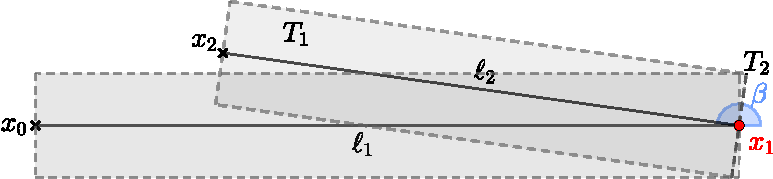
\includegraphics[width=1.0\textwidth]{2D-1stOrderApproximation_rectangles_largeTA_smalll2-crop}
	\caption[Case 2: A large turning-angle and a small step]{Case 2: A large turning-angle and a relatively small $\ell_2$. The top triangle, $T_1$, and the top-right triangle, $T_2$, are labelled.}
	\label{fig:2d_model:firstorder:case2}
\end{figure}
As discussed above, case $2$ occurs when $\ell_1 \geq -  \ell_2 \cos (\beta)$. We find the area of case $2$ in a very similar way to case $1$. This time we find the area of the $\ell_2$ rectangle that does not have overlap, and this is then the newly searched area. This non-overlapping area is once again made up of two triangles, which we denote $T_1$ and $T_2$. The area of the smaller triangle, $T_2$ is
\[A_{T_2} = \frac{-r_v^2}{2} \tan(\beta). \]
The base (top edge), of the larger triangle, $T_1$, is $\ell_2 +r_v\tan(\beta)$, and so the height is
\[\tan(\pi-\beta) = h/(\ell_2+r_v\tan(\beta)) \implies h = -\ell_2 \tan(\beta)-r_v \tan^2(\beta). \]
Therefore, the area of $T_1$ is
\begin{align*}
A_{T_1} &=(\ell_2+r_v\tan(\beta))(-\ell_2 \tan(\beta)-r_v\tan^2(\beta))/2\\ 
&= \frac{-\left(\ell_2^2 \tan(\beta) + 2r_v\ell_2 \tan^2(\beta)+ r_v^2\tan^3(\beta)\right)}{2}.
\end{align*}
The total area of overlap is therefore
\begin{align*}
A_{\text{overlap}} &= 2 r_v \ell_2 - A_{T_1} - A_{T_2}\\
&=\frac{\ell_2^2 \tan(\beta) + 2r_v \ell_2(2+\tan^2(\beta))  + r_v^2 \tan^3(\beta)}{2}.
\end{align*}

In this case, the threshold angle at which this case changes to case $3$ will also be different. As can be seen in \cref{fig:2d_model:firstorder:case2}, when the height of the unshaded triangle is greater than $2r_v$, case $2$ becomes case $3$. Since this unshaded section has hypotenuse $\ell_2$ and bottom-right angle $\pi-\beta$, we get that the height is $\ell_2 \sin(\beta)$, and so the threshold angle will be
\[\beta^* = \pi-\arcsin\left(\frac{2r_v}{\ell_2}\right).\]
and so case $2$ occurs when $\pi-\arcsin\left(\frac{2r_v}{\ell_2}\right) \leq \beta \leq \pi$ and $\ell_1 \geq -  \ell_2 \cos (\beta)$.

For angles greater than $\pi$, we get a mirror of case $2$, which occurs when $\pi \leq \beta \leq \pi +\arcsin\left(\frac{2r_v}{\ell_2}\right) $ and $\ell_1 \geq -  \ell_2 \cos (\beta)$. The area for this case will be
\[A_{\text{overlap}} =\frac{-\ell_2^2 \tan(\beta) + 2r_v \ell_2(2+\tan^2(\beta))  - r_v^2 \tan^3(\beta)}{2},\]
where we have changed the sign of $\tan$ from the original expression, as we did for case $1$.

We can combine case $2$ and its mirror, by taking absolute values of $\tan(\beta)$, giving
\[  A_{\text{overlap}} = \frac{-\ell_2^2 \left|\tan(\beta)\right| + 2r_v \ell_2(2+\tan^2(\beta))  - r_v^2 \left|\tan^3(\beta)\right|}{2},\]
for $\pi-\arcsin\left(\frac{2r_v}{\ell_2}\right) \leq \beta \leq \pi+\arcsin\left(\frac{2r_v}{\ell_2}\right)$, and $\ell_2 \geq -  \ell_1 \cos (\beta)$.
\FloatBarrier
\paragraph{Case 3: Medium turning-angle}
\FloatBarrier
\begin{figure}[h!]
	\centering
	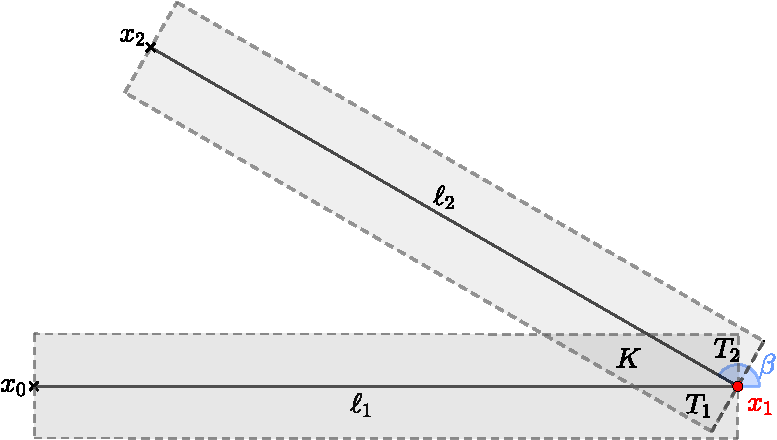
\includegraphics[width=1.0\textwidth]{2D-1stOrderApproximation_rectangles_mediumTA-crop}
	\caption[Case 3: A medium turning-angle]{Case 3: A medium turning-angle. The overlapping area is made up of a right-angled triangle at the top, $T_1$, a kite, $K$, and a right-angled triangle at the bottom, $T_2$.}
	\label{fig:2d_model:firstorder:case3}
\end{figure}

For medium-sized turning-angles, substantially less overlap may occur, depending on the size of the angle. Looking at \cref{fig:2d_model:firstorder:case3}, we see that the overlapping region is made up of three separate shapes, a right-angle triangle in the top right, a parallelogram, and a right-angle triangle at the bottom, and we denote these as $T_1$, $P$, and $T_2$, respectively. Both triangles have the same area, as we will now show. The angle of $T_1$ at $x_1$ is clearly $\beta - \pi/2$, and so is the angle of $T_2$ at $x_1$. The length of the adjacent side to this angle for both triangles must be $r_v$. Then, the length of the opposite side will be 
\[r_v \tan (\beta - \pi/2) = -r_v \cot(\beta). \]
Thus, we get
\[A_{T_1} = A_{T_2} = \frac{-r_v^2}{2} \cot(\beta). \]
For the parallelogram, the bottom and the right edge are the hypotenuse for the bottom and top triangles, respectively. Thus, the edges each have length
\[\sqrt{ r_v^2 + r_v^2 \cot^2(\beta)    } = r_v \sqrt{1+ \cot^2(\beta)} = r_v \csc(\beta). \]
The angle between these edges is $\pi - \beta$, and so the total area of the parallelogram is
\[A_k = r_v^2 \csc^2(\beta) \sin(\pi - \beta)  = r_v^2 \csc(\beta).\]
Combining the three shapes give a total overlapping area of
\[A_{\text{overlap}} = A_{T_1} + A_k + A_{T_2} = r_v^2 \csc(\beta)-r_v^2 \cot(\beta) = r_v^2 \left( \csc(\beta) - \cot(\beta)\right). \]
We can further rearrange this to get
\[A_{\text{overlap}} =  \frac{r_v^2 \sin(\beta)}{1+\cos(\beta)}. \]
However, we need to keep in mind that the sign of the trigonometric functions may change throughout the range of $\beta$ for case $3$. To ensure this doesn't happen, we rewrite our expression as
\[A_{\text{overlap}} =  \frac{r_v^2 \left|\sin(\beta)\right|}{1-\left|\cos(\beta) \right|}. \]
This expression for the area is valid for the range $\pi/2 \leq \beta \leq \pi +\arctan\left(\frac{-3r_v}{\ell_2}\right)$.

This expression is also valid for the mirrored case when $\pi -\arctan\left(\frac{-3r_v}{\ell_2}\right) \leq \beta \leq 3\pi/2$.
\FloatBarrier
\paragraph{Case 4: Small turning-angle}
\begin{figure}[h!]
	\centering
	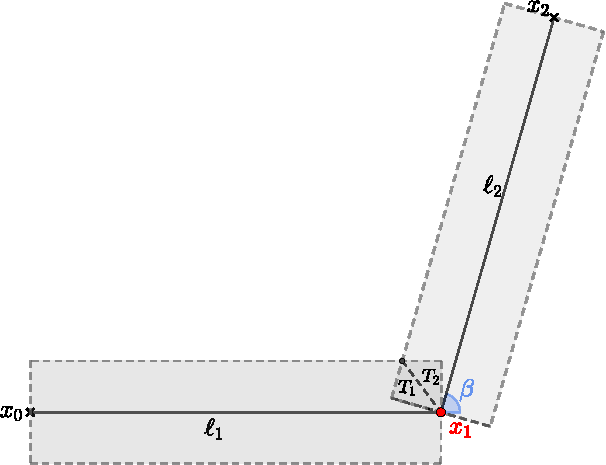
\includegraphics[width=0.8\textwidth]{2D-1stOrderApproximation_rectangles_smallTA-crop}
	\caption[Case 4: A small turning-angle]{Case 4: A small turning-angle. The overlapping area is made up of a quadrilateral, which we treat as two back-to-back right-angled triangles, $T_1$ and $T_2$.}
	\label{fig:2d_model:firstorder:case4}
\end{figure}
\FloatBarrier

When the turning angle is small, $0 \leq \beta \leq \pi/2$, only a very small amount of overlap will occur, as can be seen in \cref{fig:2d_model:firstorder:case4}. Since we require that $\lmin \geq r_v$, the length of $\ell_1$ and $\ell_2$ will not effect the overlap area for this case. The overlapping area is comprised of a kite, which in this case can be thought of as two right-angled triangles back-to-back. It is easy to see that the top-left angle of the quadrilateral will be $\pi -\beta$, and so the top-left angle for each of the two triangles will be $\pi/2 - \beta/2$. The length of the side opposite to this angle, for both triangles, is $r_v$. Therefore, the length of the adjacent side for both triangles will be
\begin{equation*}
\frac{r_v}{\tan(\pi/2-\beta/2)} = \frac{r_v}{\cot(\beta/2)} = r_v \tan(\beta/2).
\end{equation*}
Then, the total overlapping area will be the sum of the area of both triangles,
\begin{equation*}
A_{\text{overlap}} = r_v^2 \tan(\beta/2).
\end{equation*}
When making a small turn in the opposite direction, $-\pi/2 \leq \beta \leq 0$, we switch the sign of $\tan(\beta)$ to get
\begin{equation*}
A_{\text{overlap}} = -r_v^2 \tan(\beta/2).
\end{equation*}

\paragraph{Combining the four cases}
Combining each of the four cases, when $\ell_1 \geq -\ell_2 \cos(\beta)$,  the total area of overlap is
\begin{equation*}
A_{\text{overlap}} = 
\begin{cases}
r_v^2 \left|\tan(\beta/2)\right| \quad &\text{if } \beta \leq \pi/2, \text{ or } \beta \geq 3\pi/2,\\\\
\displaystyle \frac{r_v^2 \left|\sin(\beta)\right|}{1-\left|\cos(\beta) \right|} &\text{if } \pi/2  \leq \beta \leq  \pi-\arcsin\left( \frac{2r_v}{\ell_2} \right),\\
&\text{or }\pi+\arcsin\left( \frac{2r_v}{\ell_2} \right) \leq \beta \leq 3\pi/2,\\\\
\displaystyle \frac{1}{2} \left[-\ell_2^2 \left|\tan(\beta)\right| + 2r_v \ell_2(2+\tan^2(\beta))\right.  &\text{if }\pi-\arcsin\left( \frac{2r_v}{\ell_2} \right) \leq \beta,\\
\left.  - r_v^2 \left|\tan^3(\beta)\right| \right]   &\text{and } \beta \leq \pi +\arcsin\left( \frac{2r_v}{\ell_2} \right),
\end{cases}
\end{equation*}
and when $\ell_1  < -\ell_2 \cos(\beta)$, the overlap is
\begin{equation*}
A_{\text{overlap}} = 
\begin{cases}
r_v^2 \left|\tan(\beta/2)\right| \quad &\text{if } \beta \leq \pi/2, \text{ or } \beta \geq 3\pi/2,\\\\
\displaystyle \frac{r_v^2 \left|\sin(\beta)\right|}{1-\left|\cos(\beta) \right|} &\text{if } \pi/2  \leq \beta \leq  \pi+\arctan\left( \frac{-3r_v}{\ell_1} \right),\\
&\text{or }\pi-\arctan\left( \frac{-3r_v}{\ell_1} \right) \leq \beta \leq 3\pi/2,\\\\
\displaystyle \frac{1}{2} \left[-\ell_1^2 \left|\tan(\beta)\right| + 2r_v \ell_1(2+\tan^2(\beta))\right.   &\text{if }\pi+\arctan\left( \frac{-3r_v}{\ell_1} \right) \leq \beta,\\
\left.- r_v^2 \left|\tan^3(\beta)\right| \right]   &\text{and } \beta \leq \pi -\arctan\left( \frac{-3r_v}{\ell_1} \right).
\end{cases}
\end{equation*}

The angles at which the expressions change depend on the length of the steps, and the lengths at which the expressions change depend on the angle. To get around this, we simplify our expressions by replacing the condition $\ell_1 < -\ell_2 \cos(\beta)$ with $\ell_1 < \ell_2$, introducing another small amount of error. Now, note that when $\ell_1 \approx \ell_2$ and $\ell_2 \gg r_v$, then $\arctan\left( \frac{-3r_v}{\ell_1}\right) \approx -\arcsin\left( \frac{2r_v}{\min(\ell_1,\ell_2)} \right)$. Thus, the function for the overlapping area becomes
\begin{equation*}
A_{\text{overlap}} = 
\begin{cases}
r_v^2 \left|\tan(\beta/2)\right| \quad &\text{if } \beta \leq \pi/2 \text{ or } \beta \geq 3\pi/2,\\\\
\displaystyle \frac{r_v^2 \left|\sin(\beta)\right|}{1-\left|\cos(\beta) \right|} &\text{if } \pi/2  \leq \beta \leq  \pi-\arcsin\left( \frac{2r_v}{\min(\ell_1,\ell_2)} \right),\\
&\text{or }\pi+\arcsin\left( \frac{2r_v}{\min(\ell_1,\ell_2)} \right) \leq \beta \leq 3\pi/2\\\\
\displaystyle \frac{1}{2} \left[-\min(\ell_1,\ell_2)^2 \left|\tan(\beta)\right| \right. &\text{if }\pi-\arcsin\left( \frac{2r_v}{\min(\ell_1,\ell_2)} \right) \leq \beta\\
\left.+ 2r_v \min(\ell_1,\ell_2)(2+\tan^2(\beta))\right.  &\text{and } \beta \leq \pi +\arcsin\left( \frac{2r_v}{\min(\ell_1,\ell_2)} \right).\\
\left. - r_v^2 \left|\tan^3(\beta)\right| \right]   
\end{cases}
\end{equation*}

Then, the total area covered by a step of length $\ell_2$, and with turning-angle $\beta$, with previous step-length $\ell_1$ will be
\begin{equation*}
A = 2\ell_2 r_v - A_{\text{overlap}}.
\end{equation*}